Пусть \( (\Omega, \F, P) \)~--- вероятностное пространство, \(\xi:\; \Omega \rightarrow \mathbb{R}\)~--- случайная величина.

Определим матожидание 

\[\E \xi = \int_{\Omega} \xi dP \xlongequal[x = \xi(\omega)]{\text{теорема о замене переменных}} \int_{\mathbb{R}} x d\Pxi.\]

Причем если интеграла не существует, то не существует и мат. ожидания. Мат ожидание может быть бесконечным. Определим такие случаи.

Определим
\[ \xi = \xi^+ - \xi^-,\quad \xi^+ = \max{(\xi, 0)},\;\; \xi^- = \max{(-\xi, 0)}.\]

Тогда
\begin{itemize}
    \item \(\int{\xi^+ dP < \infty},\; \int{\xi^- dP < \infty} \implies |\E{\xi}| < \infty\)
    \item \(\int{\xi^+ dP = \infty},\; \int{\xi^- dP < \infty} \implies \E{\xi} = +\infty\)
    \item \(\int{\xi^+ dP < \infty},\; \int{\xi^- dP = \infty} \implies \E{\xi} = -\infty\)
\end{itemize}

\subsubsection*{Случай \texorpdfstring{$\xi$}{кси}~--- дискретная}
Тогда носитель $X$~--- не более чем счётный: \(\Pxi (X) = 1\). В таком случае
\[\E \xi = \sum_{x \in X} xP(\xi = x).\]

\subsubsection*{Примеры}

\begin{enumerate}
    \item \(\xi \sim Bern(p), \; \pxi(\{1\}) = p, \pxi(\{0\}) = 1 - p\).
    \[\E \xi = p.\]
    \item \(\xi \sim Bin(n, p), \; \pxi(\{k\}) = C^k_n p^k (1-p)^{n-k}\).
    \begin{align*}
        \E \xi &= \sum_{k = 0}^n {k C^k_n p^k (1-p)^{n-k}}\\
        &= \sum_{k = 0}^n {\frac{n!}{(k-1)! (n-k)!}p^k (1-p)^{n-k}} = np\sum_{k = 1}^n {C_{n-1}^{k-1} p^{k-1} (1-p)^{n-k}}\\
        &= np (p + (1-p))^{n-1} = np
    \end{align*}
    \item \(\xi \sim Pois(\lambda), \; \pxi (\{k\}) = \frac{\lambda^k e^{-\lambda}}{k!}, k \in \mathbb{Z_+}\).
    \begin{align*}
        \E \xi = \sum_{k = 0}^{\infty}{k \frac{\lambda^k e^{-\lambda}}{k!}} &= \sum_{k = 0}^{\infty}{ \frac{\lambda^k e^{-\lambda}}{(k-1)!}}\\
        &= \lambda e^{-\lambda} \sum_{k = 1}^{\infty} \frac{\lambda^{k-1}}{(k-1)!} = \lambda e^{-\lambda} e^{\lambda} = \lambda.
    \end{align*}
\end{enumerate}

\subsubsection*{Случай \texorpdfstring{$\xi$}{кси}~--- абсолютно непрерывная}
В этом случае
\[\E\xi = \int_{\R}x \pxi(x) dx.\]

\begin{statement}
Если \(g:\R \rightarrow \R\)~--- бореллевская и $\Pxi$~--- абсолютно непрерывна, то
\[\int g(x)d\Pxi = \int g(x) \pxi(x) dx.\]
\end{statement}

\begin{proof}
Рассмотрим случаи.
\begin{enumerate}
    \item Если индикатор $g(x) = I(x \in B),\; B \in \B(\R)$, то 
    \begin{align*}
        \int_{\R} g(x) d\Pxi = \int_{B}d\Pxi = \Pxi(B)
        = \int_{B}\pxi(x) dx = \int_{\R} g(x) \pxi(x) dx.
    \end{align*}
    \item Если простая функция \(g(x) = \sum_{i=1}^n g_i I(x \in B_i),\; B_i \in \B(\R)\), то
    \begin{align*}
        \int_{\R}g(x) d\Pxi = \sum_{i = 1}^n g_i \int_{\R}I(x \in B_i) d\Pxi = \sum_{i = 1}^n g_i  \int_{\R}I(x \in B_i) \pxi(x) dx = \int_{\R} g(x) \pxi(x) dx.
    \end{align*}
    \item Если $g \geqslant 0$, то существует последовательность простых функций \(0 \leqslant g_n,\; g_n\uparrow g\). В таком случае
    \begin{align*}
        \int_\R{g(x) d\Pxi} = \lim_{n \rightarrow \infty} \int_\R g_n(x) d\Pxi =  \lim_{n \rightarrow \infty} \int_\R g_n(x) \pxi(x) dx = \int_\R {g(x) \pxi(x) dx}
    \end{align*}
    \item Случай произвольной \(g = g^+ - g^-\):
    \begin{align*}
        \int g(x) d\Pxi &= \int g^+(x) d\Pxi - \int g^-(x) d\Pxi \\
        &= \int g^+(x)\pxi dx - \int g^-(x)\pxi dx \\
        &= \int g(x)\pxi dx
    \end{align*}
\end{enumerate}
\end{proof}

\subsubsection*{Примеры}
\noindent 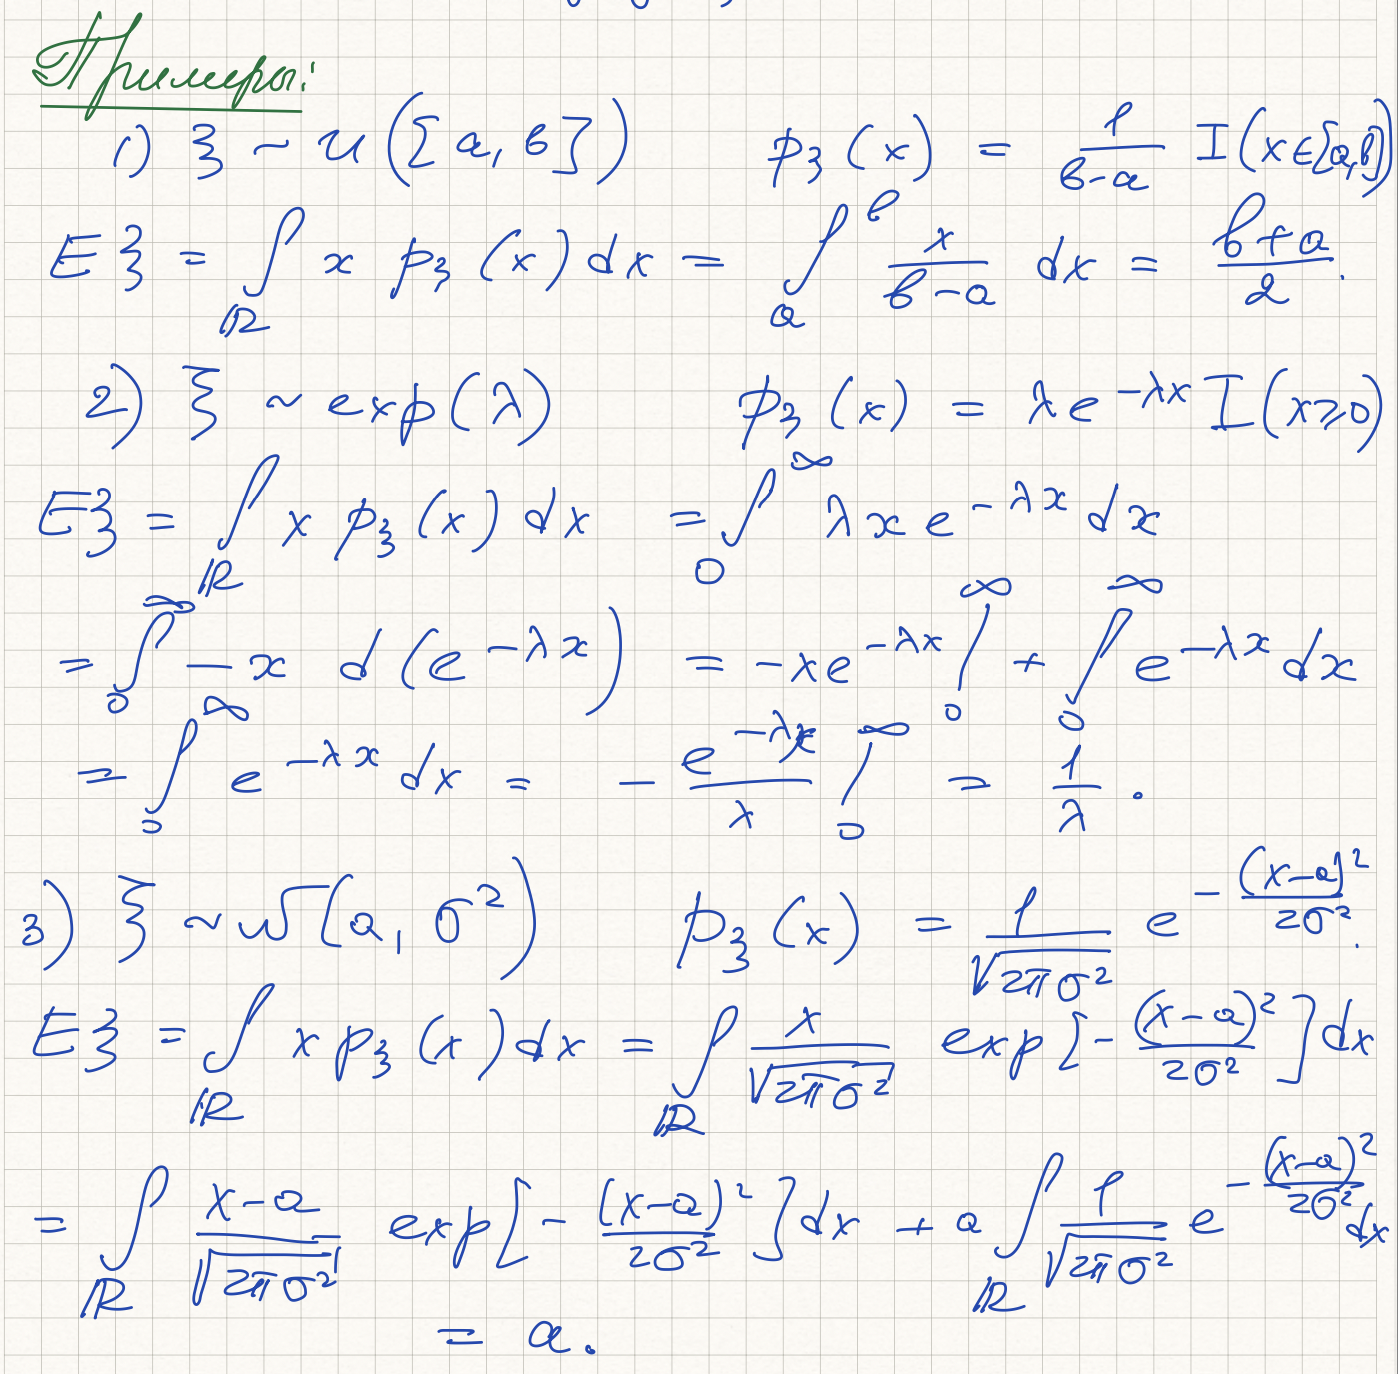
\includegraphics[width=1\linewidth]{sections/sasha/images/expect-examples.png}

\subsubsection*{Свойства мат. ожидания}
\begin{trait}
    \(\forall a \in \R \;:\; \E a\xi = a\cdot\E\xi\)
\end{trait}

\begin{trait}
\label{trait-mathexp-2}
    Если
    \(\xi \geqslant 0\), то \( \E\xi \geqslant 0\)
    
    \hspace{14ex} Если \(\xi \geqslant 0, \E\xi = 0 \), то \( P(\xi = 0) = 1\)
\end{trait}
\begin{proof}
        Так как $\xi \geqslant 0$, то существует последовательность неотриц. простых $\xi_n \uparrow \xi$\\
        Т.к. $\xi_n \leqslant \xi$, то $\E\xi_n \leqslant \E\xi = 0$. Откуда $\E\xi_n = 0$.
        \[\E\xi_n = \sum a_k P(\xi_n \in B_k) = 0.\]
        Значит, $a_k = 0 \implies \xi_n = 0$. Следовательно, $P(\xi = 0) = 1$.
\end{proof}

\begin{trait}
Если $\xi > \eta$ и $\E\xi, \E\eta$ существуют, то $\E\xi \geqslant \E\eta$
\end{trait}
\begin{proof}
    \(\xi - \eta \geqslant 0 \;\Rightarrow \; \E(\xi - \eta) \geqslant 0\), а значит по линейности \( \E\xi  - \E\eta \geqslant 0\)
\end{proof}

\begin{trait}
Если существует $\E\xi$, то $\forall A \in \F$ существует $\E(\xi I_A)$

\hspace{14.8ex}Если $|\E\xi|\, < \infty$, то $\forall A \in \F \; \E(\xi I_A) < \infty$.
\end{trait}
\begin{proof}
    Существует $\E\xi$, то либо $\E\xi^+ < \infty$, либо $\E\xi^- < \infty$
    
    Без ограничения общности пусть $\E\xi^+ < \infty$. Распишем:
    \[\xi I_A = (\xi^+ - \xi^-) I_A = \xi^+ I_A - \xi^- I_A =  (\xi I_A)^+ - (\xi I_A)^-\]
    
    Так как $\xi^+ I_A \leqslant \xi^+$, то $\E\xi^+ I_A \leqslant \infty$. Значит, $\E\xi I_A$ существует.
    
    Доказательство в случае $|\E\xi| < \infty$ аналогично.
\end{proof}

\begin{trait}
Если существует $\E\xi$, то $|\E\xi| \leqslant \E|\xi|$
\end{trait}

\begin{trait}
Если существует $\E\xi$, то \[\forall c \in \R\; \E(c\xi) = c \E\xi\]
\end{trait}

\begin{trait}[Линейность]
Если существует $\E\xi, \E\eta$ существуют и если оба бесконечны, то одинаковых знаков, то 
\[\E(\xi + \eta) = \E\xi + \E\xi\]
\end{trait}

\begin{trait}\label{exp-trait-nine}
Пусть $|\E\xi|, |\E\eta| < \infty$ и $\forall A \in \F$
\[
\E \xi I_A \leqslant \E\eta I_A,
\]
тогда 
\[P(\xi \leqslant \eta) = 1.\]
\end{trait}
\begin{proof}
    Введём \(A = \{\omega: \xi(\omega) > \eta(\omega)\} \in \F\). Перепишем условие:
    \[\E \xi I_A \leqslant \E\eta I_A \implies \E(\eta - \xi) I_A \geqslant 0.\]
    
    Причём $(\eta - \xi) I_A = 0$ при $\xi \leqslant \eta$ и 
    $(\eta - \xi) I_A < 0$ при $\xi > \eta$.
    
    Тогда, $(\eta - \xi) I_A$ неположительная случайная величина и значит мат. ожидание от нее тоже не может быть положительным. С другой стороны выполнено и $\E(\eta - \xi) I_A \geqslant 0$. 
    
    Значит, $\E(\eta - \xi) I_A = 0$ и по свойству~(\ref{trait-mathexp-2}),
    $P((\eta - \xi) I_A = 0) = 1$. Но тогда $P(\xi \leqslant \eta) = 1$.
\end{proof}
\begin{trait}
\label{mathexp-trait-independ}
Если $\xi \indep \eta, \E\xi, \E\eta$~--- существуют и конечны, то $\E(\eta \xi) = \E\eta \cdot \E\xi$
\end{trait}
\begin{proof}
    Прямое следствие теоремы Фубини.
    
    \begin{align*}
        \E(\xi\eta) &= \int_{\Omega} \xi(\omega)\eta(\omega) dP\\
        &= \int_{\R^2}xy dP_{(\xi, \eta)} = \int_{\R^2}xy d(P_\xi \times P_\eta) \\
        &\xlongequal[]{\text{теорема Фубини}} \int_{\R} x dP_\xi \int_{\R} y dP_\eta = \E\eta \E\xi.
    \end{align*}
\end{proof}